\section{\Large PROBLEM SET 6}
\subsection{PROBLEM 1}
\textit{Complete the modeling and verification of perturbation torques as described in the previous pset}

We have implemented models of the drag, gravity gradient, magnetic field, and solar radiation pressure effects on our satellite. Our magnetic field model uses a fourth-order representation suitable for LEO, and we also propagate the motion of Earth around the sun for accurate determination of solar radiation pressure. Please see the relevant portions of the previous section for more detail.


\subsection{PROBLEM 2}
\textit{Compute the attitude control error even if a controller is not implemented yet. The attitude control error represents the rotation between the desired and actual attitude. Plot the attitude control error and give its interpretation. Note that this step requires the definition and computation of the desired or nominal or target attitude of the spacecraft. In general, this can be expressed in body or principal axes.}

In operation, NISAR will point its antenna towards Earth such that the principal x-axis facing the negative radial direction and the principal y-axis is pointing in the negative normal direction. The angular velocity about the principal y-axis is the negative of mean motion.
\begin{align*}
    \Vec{P}_{desired} &= 
    \begin{bmatrix}
    -1 & 0 & 0 \\
    0 & 0 & -1 \\
    0 & -1 & 0
    \end{bmatrix}
    \Vec{P}_{RTN}
\end{align*}
We first simulate attitude without disturbance torques, calculating error as the rotation between target and actual attitude. Figures \ref{fig:Images/ps6_problem2_principal}, \ref{fig:Images/ps6_problem2_target}, \ref{fig:Images/ps6_problem2_error} demonstrate that the error is approximately zero.

\begin{figure}[H]
\centering
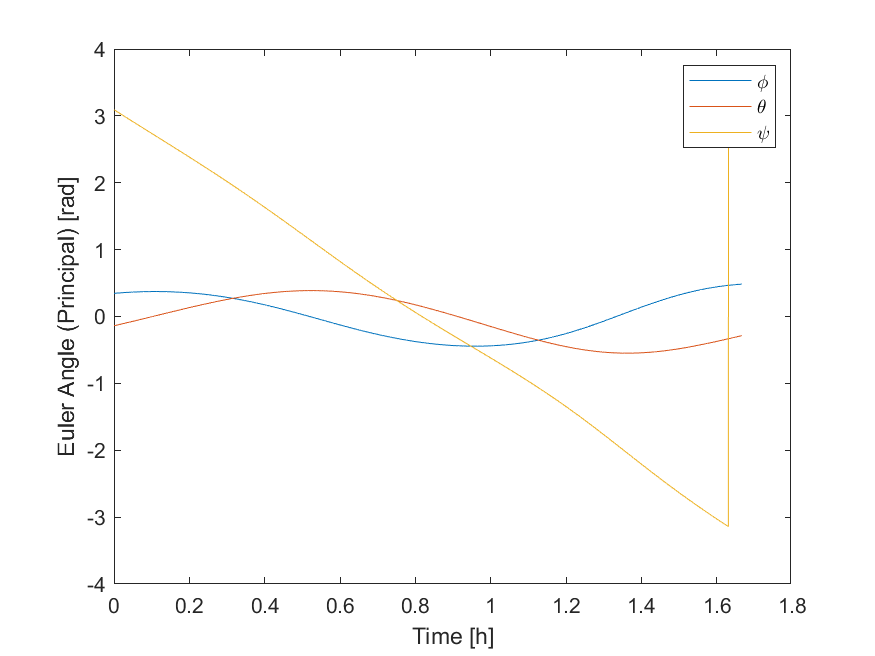
\includegraphics[scale=0.6]{Images/ps6_problem2_principal.png}
\caption{Actual attitude relative to inertial frame, without perturbations}
\label{fig:Images/ps6_problem2_principal}
\end{figure}

\begin{figure}[H]
\centering
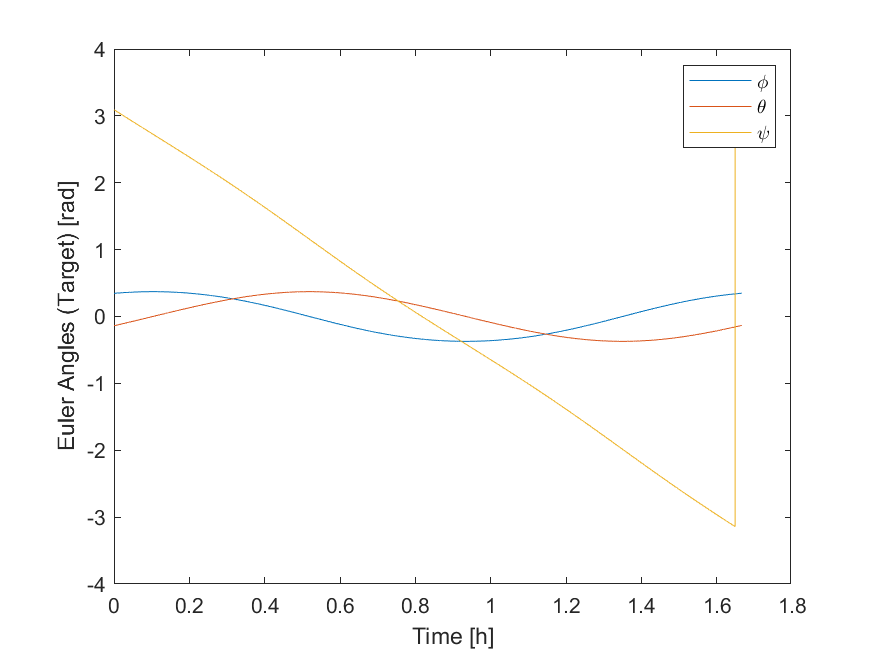
\includegraphics[scale=0.6]{Images/ps6_problem2_target.png}
\caption{Target attitude relative to inertial frame, without perturbations}
\label{fig:Images/ps6_problem2_target}
\end{figure}

\begin{figure}[H]
\centering
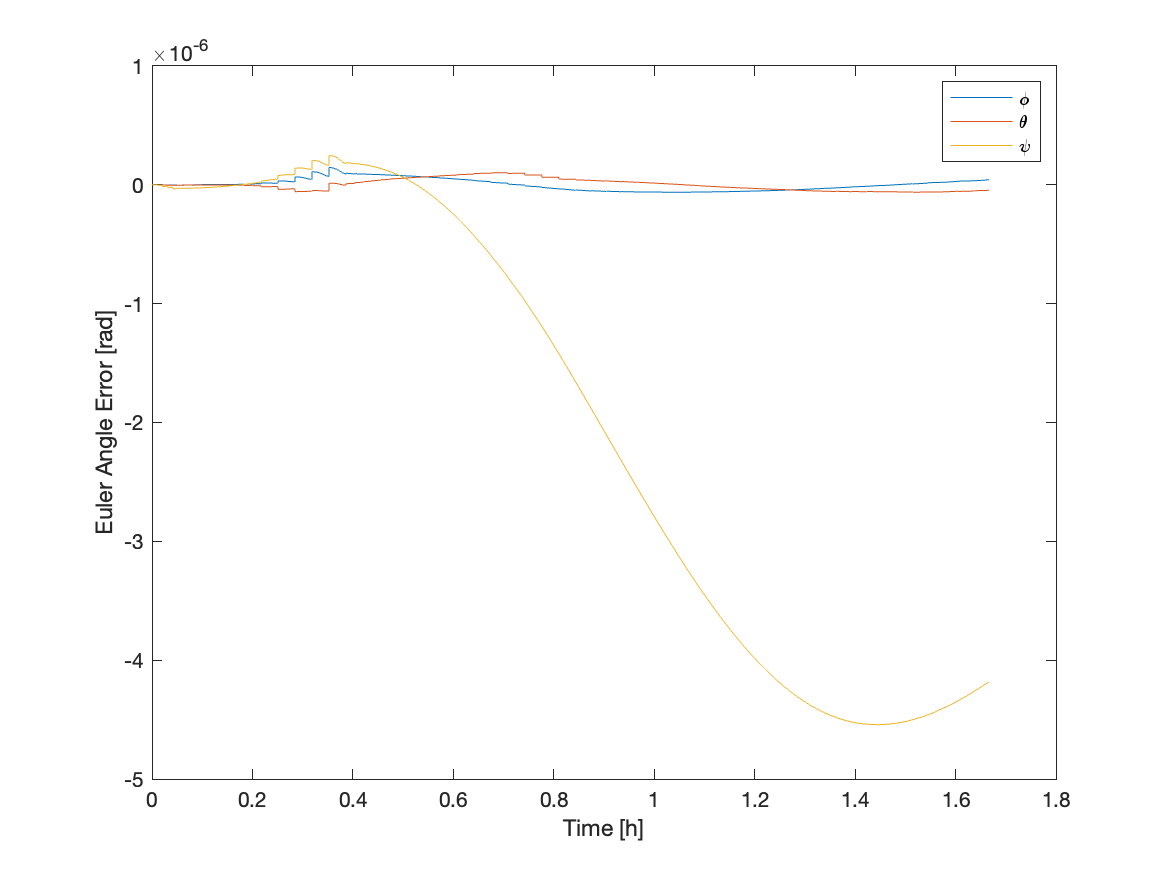
\includegraphics[scale=0.6]{Images/ps6_problem2_error.png}
\caption{Error between target and actual attitude, without perturbations}
\label{fig:Images/ps6_problem2_error}
\end{figure}

For computing errors, we multiply the DCM representing the rotation from the inertial frame to our actual attitude with the inverse of the DCM representing the rotation from the inertial frame to the target attitude. We observe that there is a very small error (approximately $10^{-7}$ to $10^{-6}$) in our result in Figure \ref{fig:Images/ps6_problem2_error}. This is most likely arising from our use of numerical integration.

\subsection{PROBLEM 3}
\textit{Note that the attitude control error represents a rotation matrix (DCM) which quantifies how far the actual attitude is from the true attitude. You can use any parameterization to plot the attitude control errors corresponding to this DCM. Give interpretation of the attitude control errors given the applied disturbances.}

With perturbations, we observe a small but noticeable change to actual attitude in Figure \ref{fig:Images/ps6_problem3_principal}.

\begin{figure}[H]
\centering
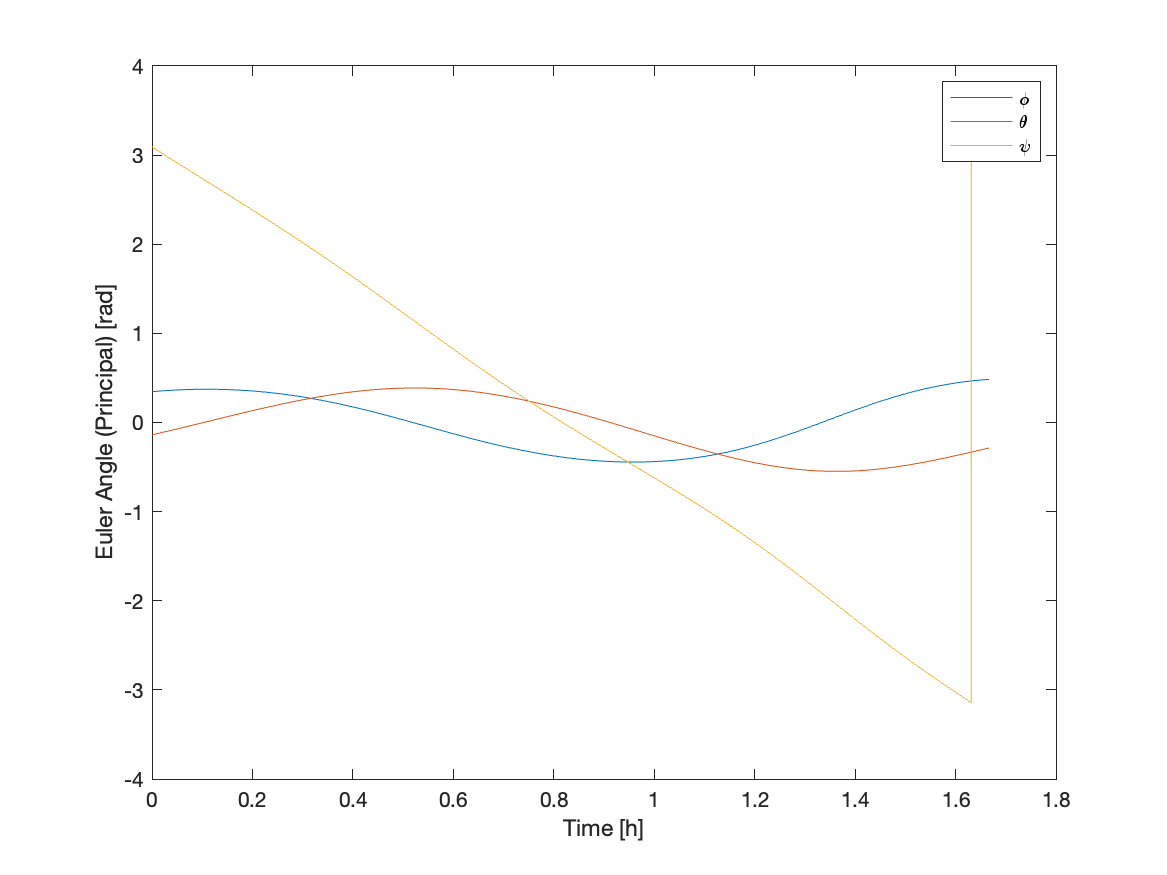
\includegraphics[scale=0.6]{Images/ps6_problem3_principal.png}
\caption{Actual attitude relative to inertial frame, with perturbations}
\label{fig:Images/ps6_problem3_principal}
\end{figure}

\begin{figure}[H]
\centering
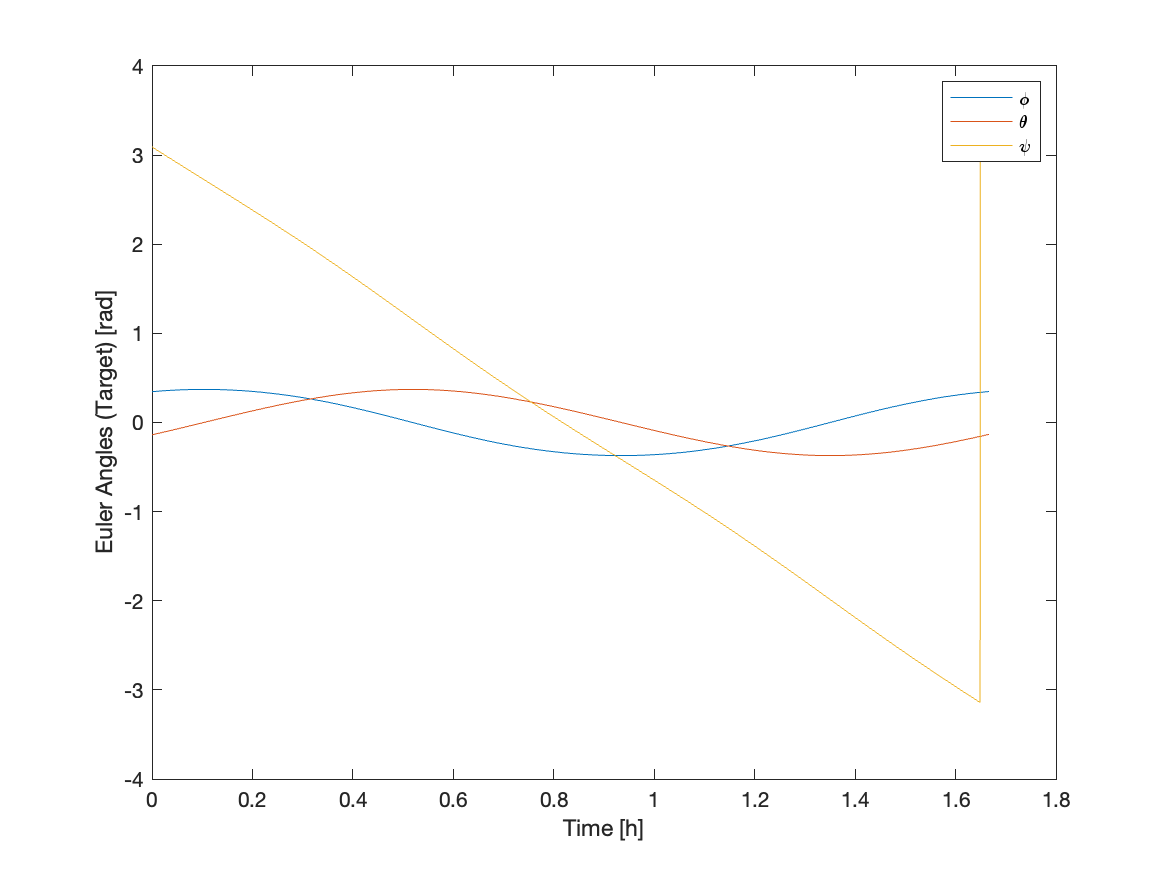
\includegraphics[scale=0.6]{Images/ps6_problem3_target.png}
\caption{Target attitude relative to inertial frame, with perturbations}
\label{fig:Images/ps6_problem3_target}
\end{figure}

A much larger error appears in Figure \ref{fig:Images/ps6_problem3_error}. When compared with the disturbance-free error in Figure \ref{fig:Images/ps6_problem2_error} (which is approximately zero), we can interpret the attitude control error as the amount which the disturbance torques rotate our satellite during the simulation period, which in this case is one orbital period.

\begin{figure}[H]
\centering
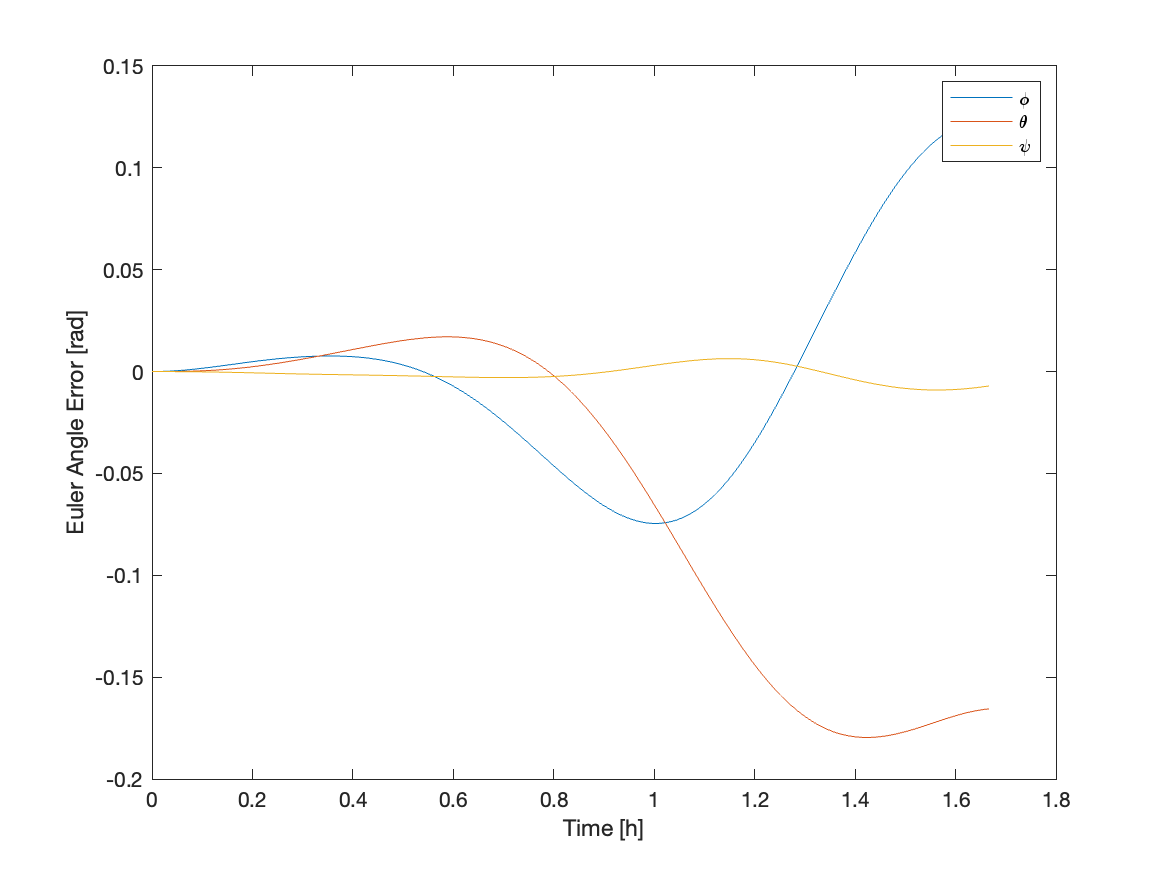
\includegraphics[scale=0.6]{Images/ps6_problem3_error.png}
\caption{Error between target and actual attitude, with perturbations}
\label{fig:Images/ps6_problem3_error}
\end{figure}

\subsection{PROBLEM 4}
\textit{You can now start modeling the Simulink spacecraft subsystem which is what the satellite believes is happening (on-board). Initially, the sensors provide ideal measurements (no bias or noise). Just use an empty box for those. The outputs of the sensors are measurements which are used for attitude determination. These measurements are computed from the reference truth or oracle.}

Five arbitrary vectors were picked to be the "ground truth." With those, the DCM matrix between ECI and the satellite's principal axes were used to get noiseless measurement readings. In the future, some noise will be added to this step, but for now it is not needed.

\subsection{PROBLEM 5}
\textit{Assume a certain set of sensors. In general, a number of unit vectors and angular velocities can be considered as measurements}

\textit{Implement the deterministic attitude determination algorithm discussed in class and its variant which uses fictitious measurements to spread the errors across the measurements}

\textit{Implement the statistical attitude determination algorithm discussed in class (q-method)}

\textit{Implement angular velocity measurements and the reconstruction of the attitude from those (through kinematic equations coded identically to ground truth but replicated in the spacecraft on-board computer)}

The methods for attitude determination were implemented in the following functions, with deterministic attitude determination having an implementation with two vectors and another with multiple readings.

\lstinputlisting{src/DAD_twoVecs.m}
\lstinputlisting{src/DAD.m}
\lstinputlisting{src/qMethod.m}
\lstinputlisting{src/kinEulerStepRK4.m}


\subsection{PROBLEM 6}
\textit{Plot the resulting estimated attitude in the absence of sensor errors. Show that it is identical to the true attitude (except for numerical errors).}

Figures \ref{fig:Images/ps6_problem6_actual}, \ref{fig:Images/ps6_problem6_DADFict}, \ref{fig:Images/ps6_problem6_DAD}, and \ref{fig:Images/ps6_problem6_qMethod} depict the attitude determination using the different methods discussed earlier. As can be seen, they all align, which makes sense given how there is no measurement error.

\begin{figure}[H]
\centering
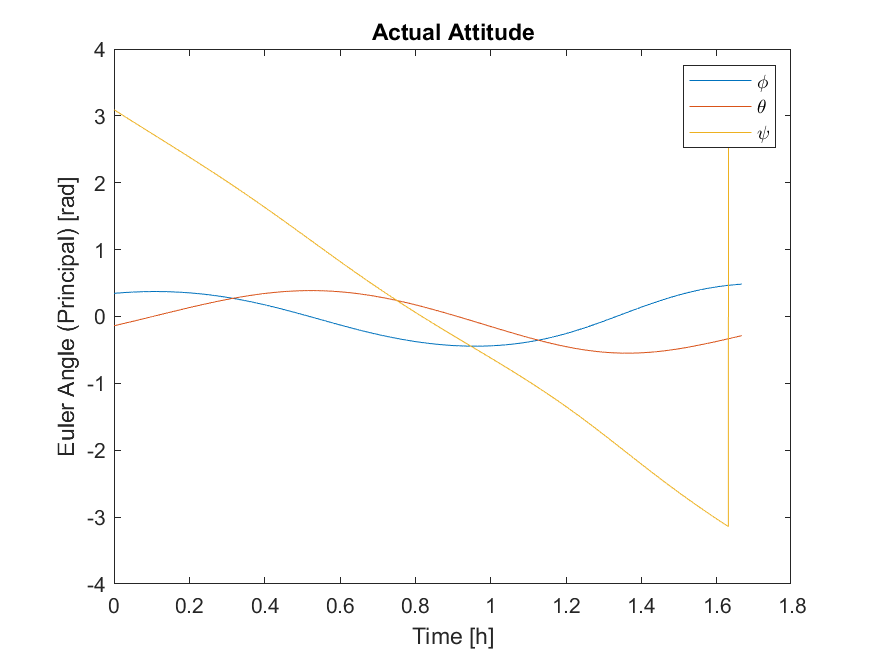
\includegraphics[scale=0.7]{Images/ps6_problem6_actual.png}
\caption{Actual satellite attitude in ideal frame}
\label{fig:Images/ps6_problem6_actual}
\end{figure}

\begin{figure}[H]
\centering
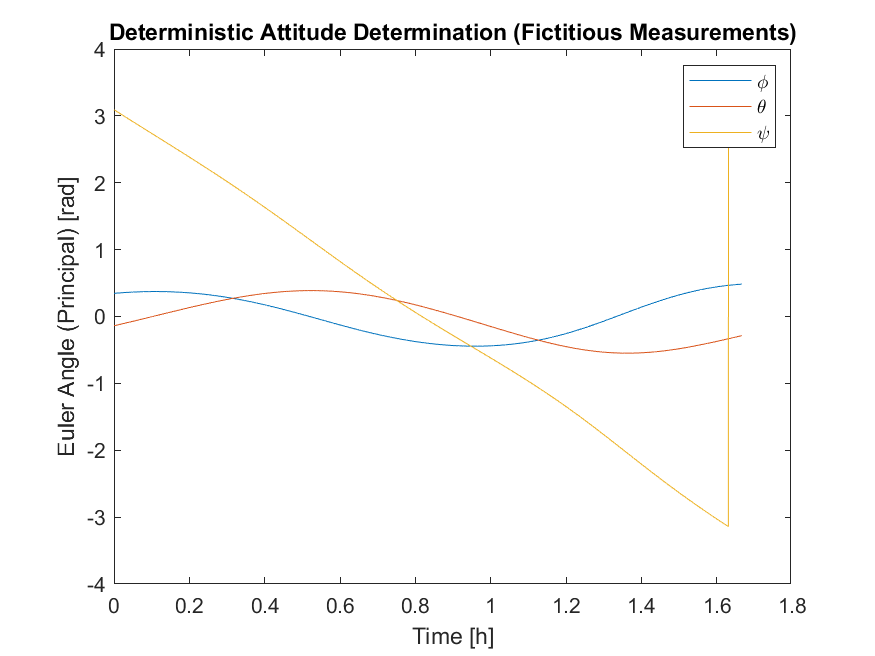
\includegraphics[scale=0.7]{Images/ps6_problem6_DADFict.png}
\caption{Attitude based on Deterministic Attitude Determination with fictitious measurements}
\label{fig:Images/ps6_problem6_DADFict}
\end{figure}

\begin{figure}[H]
\centering
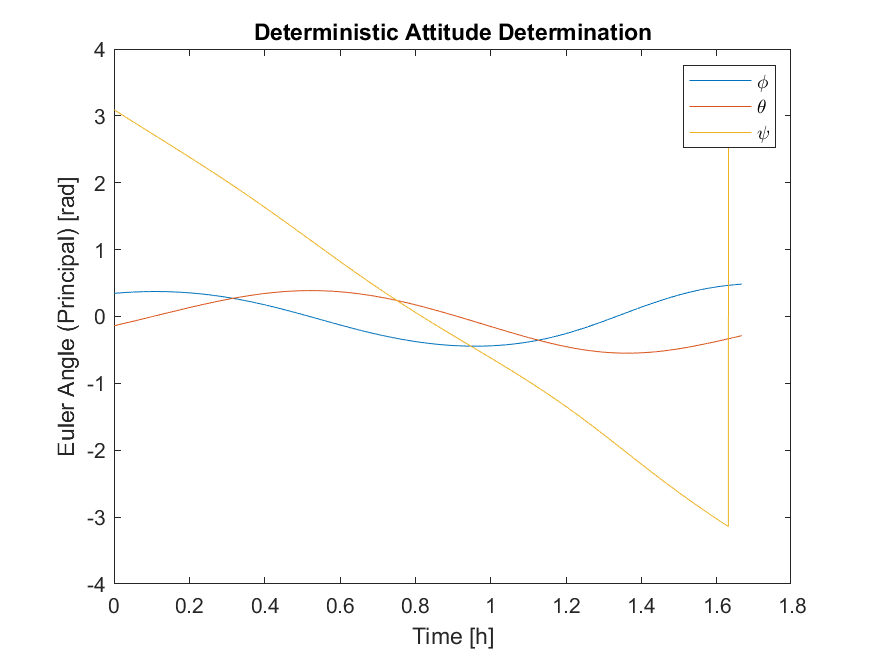
\includegraphics[scale=0.7]{Images/ps6_problem6_DAD.png}
\caption{Attitude based on Deterministic Attitude Determination with fictitious measurements}
\label{fig:Images/ps6_problem6_DAD}
\end{figure}

\begin{figure}[H]
\centering
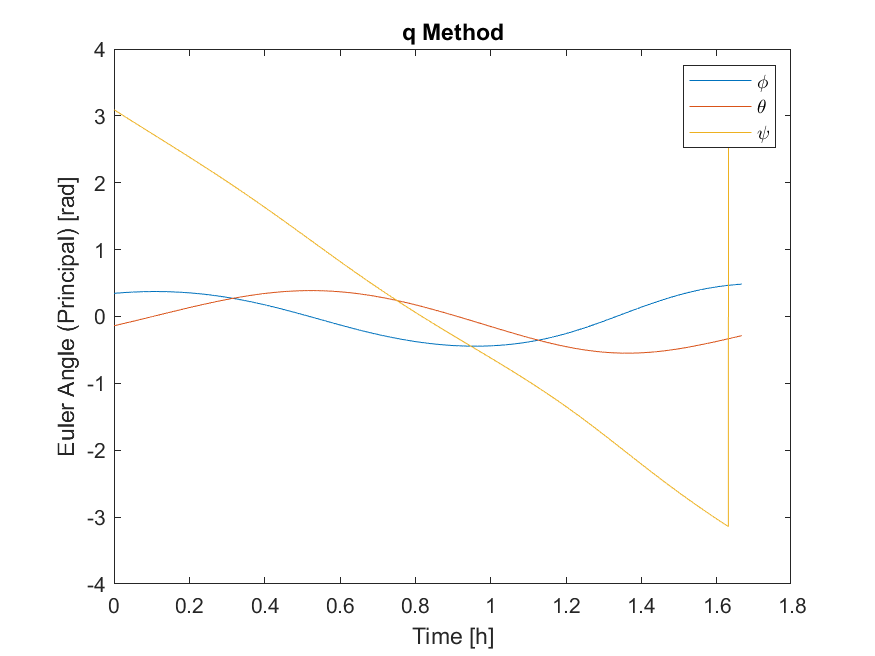
\includegraphics[scale=0.7]{Images/ps6_problem6_qMethod.png}
\caption{Attitude based on q Method}
\label{fig:Images/ps6_problem6_qMethod}
\end{figure}

\begin{figure}[H]
\centering
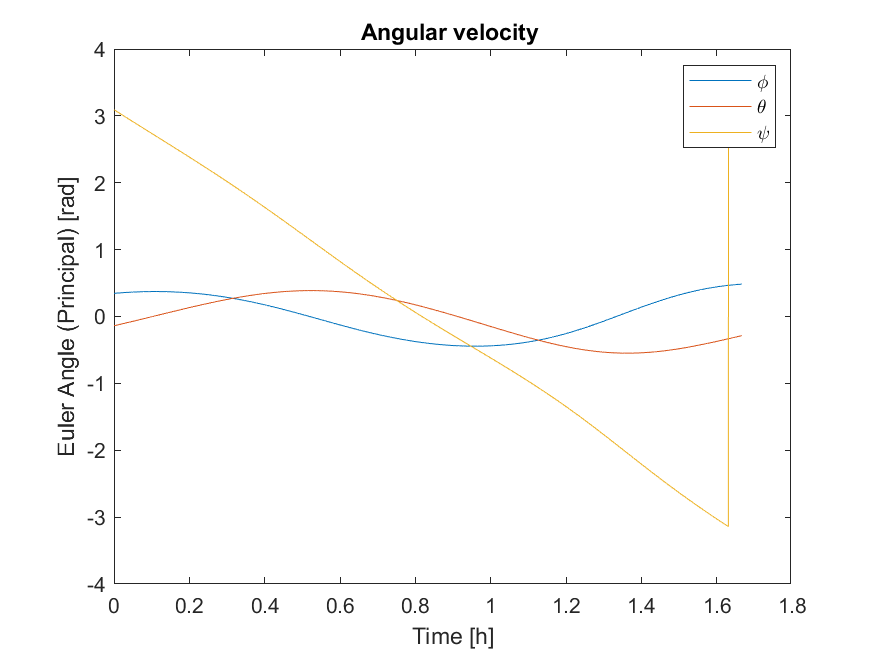
\includegraphics[scale=0.7]{Images/ps6_problem6_kins.png}
\caption{Attitude based on q Method}
\label{fig:Images/ps6_problem6_kins}
\end{figure}